\documentclass[]{article}

\usepackage{amsmath}
\usepackage{amssymb}
\usepackage{graphicx}
\usepackage{float}
\usepackage{multicol}
\usepackage{fancyhdr}
\fancyhead[L, CO] {}
\fancyhead[C, CO] {AdvContr - Résumé 2022}
\fancyhead[R, CO] {}
\usepackage[margin=1.5cm,landscape]{geometry}
\pagestyle{fancy}
\usepackage{mathtools} % for '\splitdfrac' macro
\usepackage[dvipsnames]{xcolor}
\usepackage{subfiles}
\usepackage{mdframed}
\usepackage{siunitx}

\def\Pcolor{\textcolor{RoyalBlue}}
\def\Icolor{\textcolor{OrangeRed}}
\def\Dcolor{\textcolor{ForestGreen}}
\def\Ucolor{\textcolor{Orange}}
\def\bcolor{\textcolor{RubineRed}}
\def\acolor{\textcolor{BlueViolet}}


\begin{document}
\begin{multicols}{3}
\subfile{fonction_transfert}
\subfile{espace_etats}
\subfile{regulateurs}
\subfile{nyquist}
\subfile{observateur}
\subfile{valeurs_singulieres}
\subfile{systemNonLineaire}
\subfile{incertitudes}
\subfile{identification}
\subfile{autres}
\end{multicols}
\pagebreak
\section{Exemples de réponses}
\begin{itemize}
\item \textcolor{RoyalBlue}{Réponse indicielle}
\item \textcolor{Orange}{Réponse impulsionnelle}
\end{itemize}
\begin{center}
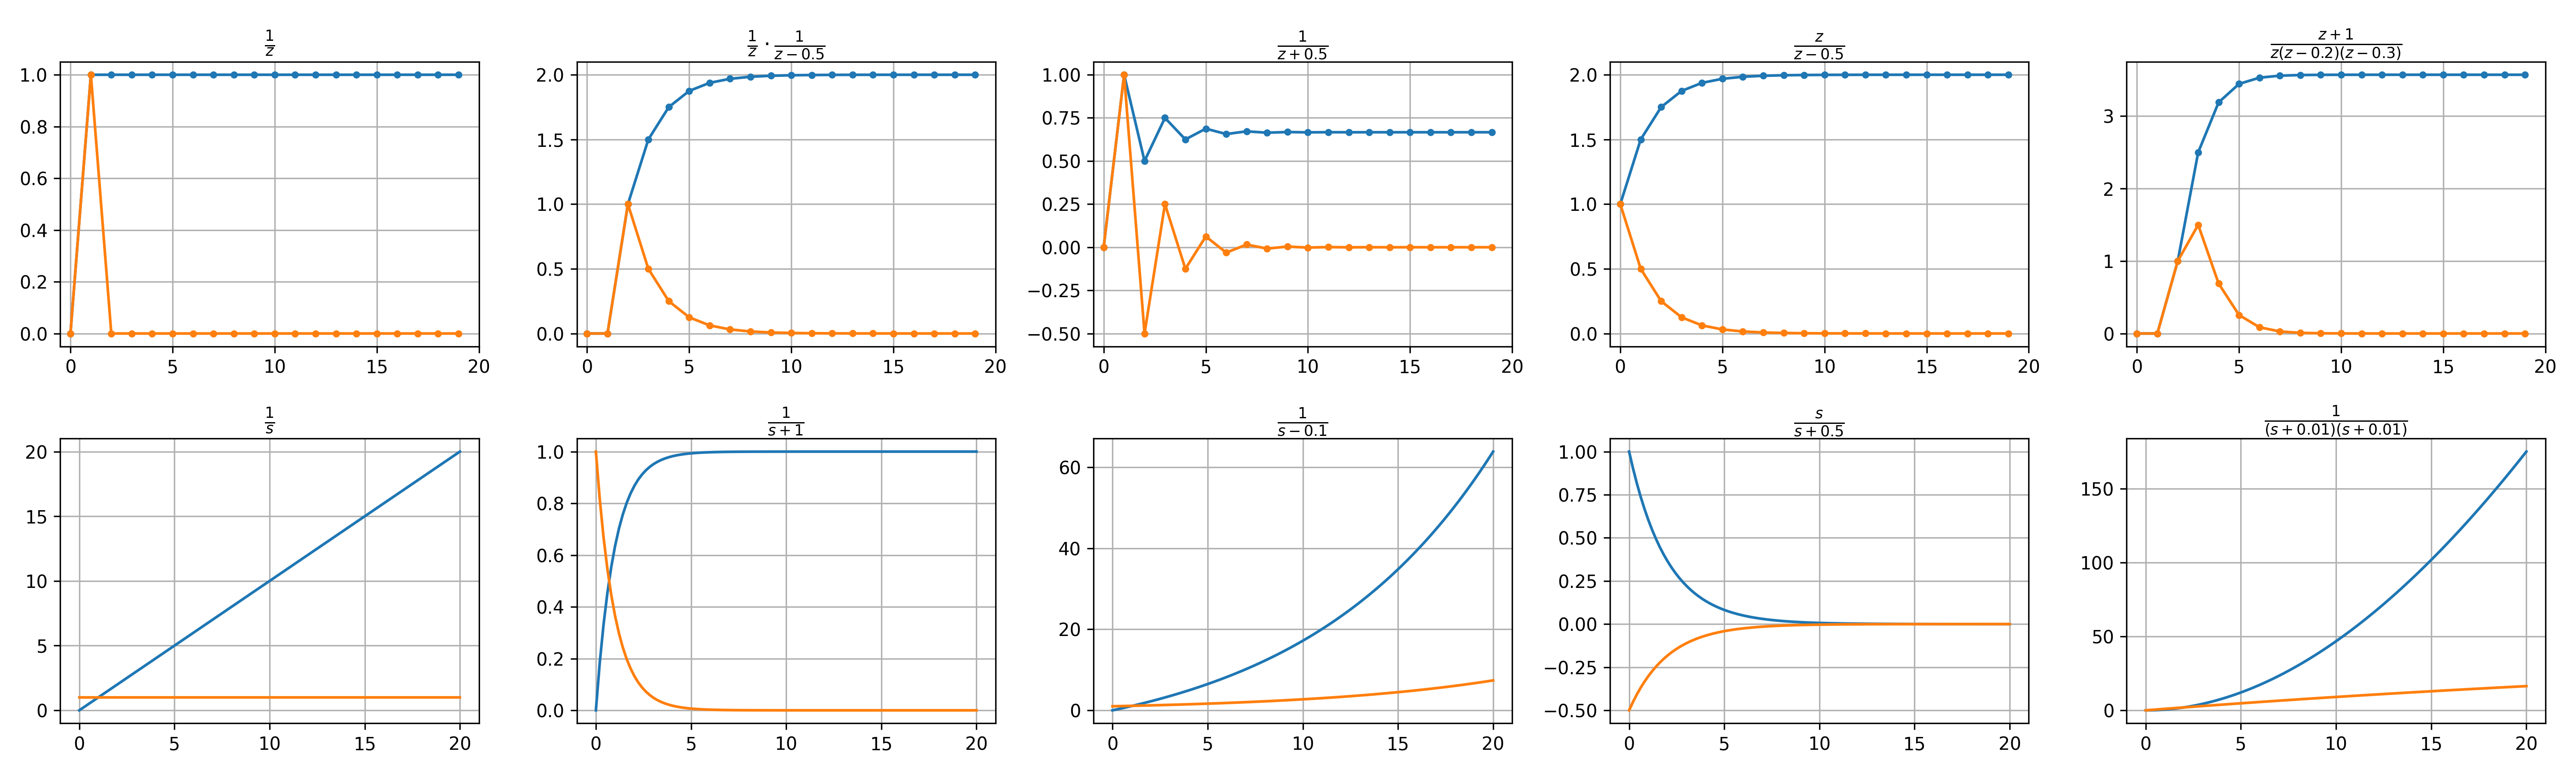
\includegraphics[width=\textwidth]{Allures.png}
\end{center}
\pagebreak
\section{Exercices}
\subsection{Série 13 - Exercice 1}
\begin{multicols}{2}
\begin{figure}[H]
\centering
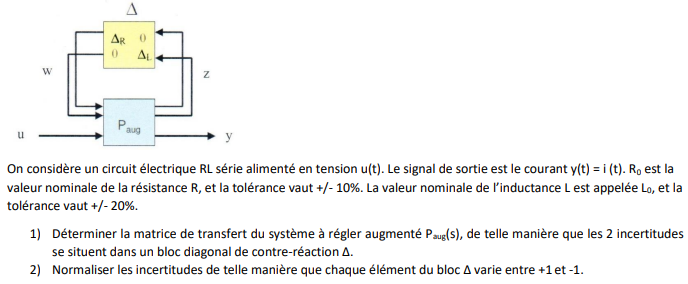
\includegraphics[width=\columnwidth]{img_12.png}
\end{figure}
\begin{figure}[H]
\centering
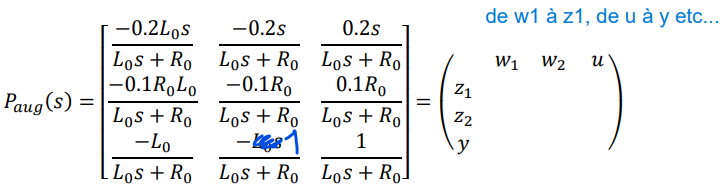
\includegraphics[width=\columnwidth]{img_15.png}
\end{figure}
\end{multicols}
\begin{figure}[H]
\centering
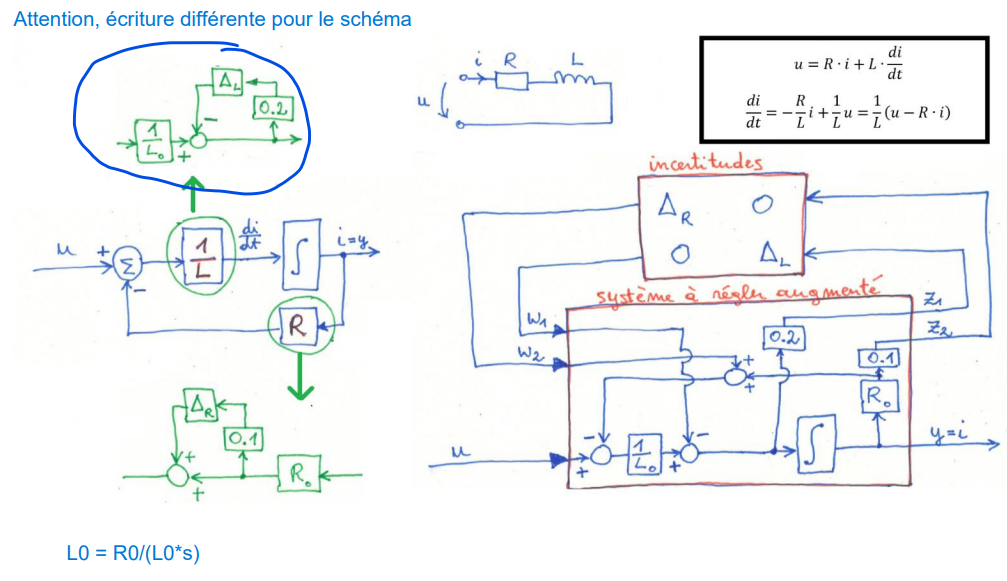
\includegraphics[width=0.7\textwidth]{img_14.png}
\end{figure}
\end{document}